\documentclass[12pt]{article}

\usepackage{amsmath}
\usepackage{graphicx}
\usepackage[margin=1in]{geometry}
\usepackage{setspace}
\usepackage[style=authoryear,backend=biber]{biblatex}
\addbibresource{impact.bib}

\begin{document}

\title{Foreign buyers and local affordability: Indications from Vancouver}
\author{Thomas Davidoff\\Sauder School of Business, UBC}
\maketitle

\onehalfspacing

\begin{abstract}

	With condominium construction paused despite severe housing affordability
	problems in Vancouver and particularly Toronto, attention has turned to
	the question of whether foreign buyer taxes may have overshot to the
	point of making affordability worse by making condo development
	unprofitable. A model that simplifies the foundational analysis in
	\textcite{favilukisVanNieuwerburgh} shows that foreign buyers help or
	hinder domestic affordability depending on whether supply is elastic or
	inelastic, whether foreign buyers overpay for units in the same
	buildings as locals, how intense foreign demand is, and whether foreign
	buyers occupy units or instead rent them to locals or flip
	preconstruction contracts near building completion. Casual data
	analysis and back-of-the-envelope calculations suggest that absent empty
	home taxes, foreign buyers in Greater Vancouver and Toronto likely
	hindered local affordability, but in the presence of empty homes taxes,
	foreign buyer bans or taxes may plausibly worsen affordability for locals.

\end{abstract}
\section{Introduction}

Taxes and restrictions on foreign purchases of residences have been implemented
in multiple jurisdictions worldwide with the stated purpose of making homes
more affordable for domestic residents. For example, in extending a ban on
foreign purchases of Canadian residential real estate, a government press
release (\textcite{gOC}) stated: ``For years, foreign money has been coming
into Canada to buy up residential real estate, increasing housing affordability
concerns in cities across the country, and particularly in major urban centres.
Foreign ownership has also fueled worries about Canadians being priced out of
housing markets in cities and towns across the country.''

There are theoretical and empirical reasons to expect foreign buyer taxes to
succeed in reducing local housing prices, many of which are detailed in a
comprehensive study by \textcite{favilukisVanNieuwerburgh}. The disincentive to
purchase homes should reduce the number of buyers considering purchasing
properties and lower willingness to pay among remaining foreign buyers. This
reduction in prices hurts landlords and incumbent property owners through lost
property value and rents, but makes home ownership more affordable for locals
who do not yet own homes. There may be an associated loss of construction jobs,
and the analysis in \textcite{favilukisVanNieuwerburgh} does not consider the
effect of reciprocal taxes on domestic residents who may wish to purchase
property overseas.\footnote{It is not obvious that a target country would wish
	to reciprocate to disincentivize the host country's tax. For example,
	China, the source of most foreign buying in Canada prior to the recent
spate of taxes (per, e.g. \textcite{ctvNews}) has made efforts to discourage capital
flight.}

In this paper, I analyze how taxes on foreign home buyers affect affordability
for locals. A simple model shows that three key parameters determine the
direction of that effect: the elasticity of housing supply with respect to
price, the extent to which foreign buyers outbid locals, and the extent to
which foreign buyers occupy homes. I gather evidence ont he magnitude of these
parameters and then use the model and likely parameter values to analyze the
conditions under which foreign housing taxes help or hurt affordability.

Existing studies of the impact of the entry and exit of foreign buyers on local home prices
present estimated effects that are all positive and range from modest to quite
large, as summarized in \textcite{davidoffZheng}. \textcite{LiShenZhang},
\textcite{gorbackGlobalCapitalLocal2020},
\textcite{pavlovImmigrationCapitalFlows2018}, and \textcite{BadarinzaRamadorai}
find that within metropolitan areas, submarkets exposed to foreign buyers see
larger price increases when the types of foreign buyers prone to buy in those
submarkets face increased incentives to buy overseas.
\textcite{DachisDurantonTurner}, \textcite{klevenBest},
\textcite{kopczukMunroe}, and \textcite{davidoffLeigh} find, as a general
matter, that increasing transaction taxes on housing purchases leads to fewer
transactions and lower prices. \textcite{HartleyForeign},
\textcite{andolfatto2024foreignbuyers}, \textcite{DuYinZhang}, and
\textcite{pavlovForeignBuyerTaxes} collectively find that foreign buyer taxes
in Australia, Canada, and New Zealand led to lower prices.
\textcite{hilber2020secondhomes} finds that banning second home construction in
desirable second home locations in Switzerland did reduce the prices of primary
residences and increased prices of second homes.

As \textcite{favilukisVanNieuwerburgh} observe, foreign buyers may not leave
homes empty, but rather rent them out to locals. In their calibration, this
changes the social welfare effect of foreign buyers from negative to slightly
positive. The positive supply effect of out of town buyers is moderate because local investors
are highly price sensitive in their demand for rental properties, and out-of-town
buyers represent a small share of overall capital investment. In this way,
foreign buyers represent a slightly positive form of capital accumulation. This
is a salient consideration, as British Columbia has imposed significant taxes on empty
homes and vacation properties in urban areas while also imposing significant
taxes on foreign buyers, and the Canadian federal government has both imposed
taxes on empty homes owned by foreigners and has temporarily banned the
purchase of single residences by foreigners.\footnote{The currently very weak state of
condo presales hints at a relatively modest supply of local
capital. Overall residential supply has not declined by as much,
likely due to significant investment from CMHC in purpose-built rental
apartment finance.}

At the time of writing, the markets for condominiums in Vancouver and Toronto
are so weak that construction has stalled, with many projects
cancelled.\footnote{\textcite{cmhc2025condominium}.} In these markets, condos
are typically financed in part by preconstruction sales (``presales'') that
commonly take place several years prior to completion of the building. While
indicative of falling prices, the ratio of condo ownership costs to incomes
remains almost at record levels per \textcite{rbc2024housing}. And the lack of
condo presales and hence starts has led some observers to suggest that the
taxation of foreign buyers has overshot, leading to a negative supply response
larger than the positive demand response on prices from foreign buying, such
that locals have been adversely affected.\footnote{See, for example,
\textcite{gold2024foreignbuyers}.} It is thus worthwhile asking whether there
is empirical evidence supporting the idea that foreign buyers, particularly in
the presence of empty homes taxes, may have positive welfare effects, and
banning or taxing foreign buyers adverse effects on housing affordability for
locals.

There are several channels through which foreign buyers could have positive
affordability effects. First, per \textcite{favilukisVanNieuwerburgh}, foreign
buyers may rent houses to locals, particularly in the presence of an empty
homes tax. Second, foreign buyers may purchase condominiums in
the presale phase of condominium development and then assign their contracts
prior to completion. The presence of foreign presale purchasers would raise
presale prices, encouraging the supply of condominiums, but with no increase in
demand for built homes. The net effect of that form of investment should be
positive for affordability for end users, with an adverse competition effect
for locals who wish to occupy homes purchased through the presale channel.

A third way in which foreign buyers could have a beneficial effect on housing
affordability for local apartment buyers if they have a relative preference for
quality, and if there is a high degree of vertical differentiation within
buildings. In that case, foreign buyers could make projects more profitable
than they would otherwise be, increasing supply, but without crowding out local
demand. This would be a positive ``pecuniary externality.'' For example, it has
been suggested that a non-trivial fraction of condo developer profits often
come from lavish penthouse units commonly sold to international buyers. If 20
floors of condos become profitable only because the 21st floor penthouse is
sold overseas, local buyers lose when the sale of that unit is banned. By
contrast, if foreign buyers compete at the same price for the same units as
local buyers, or if their purchases are concentrated in entirely different
locations, that cross-subsidy does not arise. Even a relative taste for new
construction among foreigners could improve afforability of older units for
locals, consistent with Australia's policy of exempting new construction from
foreign buyer taxes and bans.

Section \ref{sec:model} below reduces the considerations above into a single
equation governing the direction of the affordability impact of foreign buyers.
Section \ref{sec:data} reviews some available evidence on the extent to which
the channels alluded to above are operative in the Vancouver housing market,
building to some back-of-the-envelope conjectures on the net effect under
different policy regimes.

\section{\label{sec:taxes} Background: taxation and regulation of foreign buying and empty homes in Canada}

In 2016, the Province of British Columbia imposed a 15\% extra property
transfer tax on foreign (those who are not citizens, permanent residents, or
B.C. Provincial Nominees) buyers of residential property in Greater Vancouver.
That rate was subsequently expanded to other metropolitan areas in B.C. and the
rate increased to 20\%. In 2017, a similar tax was imposed on foreign buyers in
the Greater Golden Horseshoe area of Ontario.

B.C.'s foreign buyer tax legislation included a provision allowing the City of
Vancouver to impose taxes on homes not used as primary residences, with the tax
brought into effect in 2017. The tax rate has moved over time and currently
stands at 3\% of property value in each year of vacancy.\footnote{\texttt{https://vancouver.ca/home-property-development/empty-homes-tax.aspx}.} The Province of B.C.
added a similar Speculation and Vacancy tax on metropolitan areas in the
Province. That rate is higher on property owners who are foreign or earn most
of their income overseas (currently 2\%, transitioning to 3\% in 2026) than on
Canadian residents (currently .5\%, transitioning to 1\% in 2026).\footnote{See
\texttt{https://www2.gov.bc.ca/gov/content/taxes/speculation-vacancy-tax/how-tax-works/tax-rates}.}
These taxes have been matched elsewhere, including multiple jurisdictions in
Ontario, and federally, with the 2022 Underused Housing Tax, a tax of 1\% of
value, only assessed on non-primary residences owned by foreign nationals.

Effective January 1, 2023, the federal government banned foreign nationals from
purchasing residential property in Census Metropolitan Areas or Census
Agglomerations with populations greater than 10,000. That ban, initially set to
expire in 2025 has been extended to January 1, 2027.\footnote{See
\texttt{https://www.cmhc-schl.gc.ca/professionals/housing-markets-data-and-research/\\housing-research/consultations/prohibition-purchase-residential-property-non-canadians-act}.}

\section{\label{sec:model} A simple framework for evaluating foreign buyer effects on local housing affordability}

Suppose that foreign buyers have infinitely elastic demand for housing units at
a price of $p_{f}$, assumed in any relevant equilibrium greater than the
equilibrium willingness to pay among locals that comes from the demand curve
$q_{l}\left(p_{l}\right)$. The fraction of buyers that are foreign ($\alpha$ in
each building would be 100\%, but is instead determined by a government policy,
here assumed to be exogenously
chosen.\footnote{\textcite{favilukisVanNieuwerburgh} allow foreign demand to be
affected by the local price and by an time-varying exogenous factor, $\alpha$
is akin to the latter.} I ignore the distinctions among the price per unit paid
by locals $p_{l}$ the ``user cost'' per year associated with that price, and
market rent. Taxes and political preferences for one form of tenure or the
other would affect these differently.

If $\alpha>0$ and $p_{f}>p_{l}$, developers charge different prices to foreign
and local buyers. This could arise through at least two channels. First, foreign buyers
might demand higher quality units, e.g. penthouses for which they have a much
greater willingness to pay than locals, but have relatively little interest in
lower-floor, ordinary units. Relative demand for new versus older units would
have the same consequence over time. Second, developers might market a fraction
of presale units overseas, and the law of one price might not force equality of
pricing if foreign buyers are constrained in their ability to participate in
ordinary presale or resale markets.\footnote{An allegedly common practice, see,
e.g.  \textcite{citynews2017overseasbuyers}.}

The supply of housing units is given by a function $q_{s}\left(\bar{p}\right)$,
increasing in price. $\bar{p}$ is the average price at which homes are sold,
$\bar{p} \equiv \left[1-\alpha\right]p_{l} + \alpha p_{f}$.

Some fraction of housing units purchased by foreign buyers are rented out to
locals, and some presale buyers flip their homes prior to occupancy of
buildings. Call $z$ the fraction of units purchased by foreign buyers that are
unavailable to locals. The magnitude of $z$ might be
taken as a measure of how important affordable home ownership is, beyond rental
affordability. A large $z$ value could thus indicate that local consumers
renting from foreigners is seen as undesirable by policymakers, whereas $z=0$
might indicate that converting owner units to rental is not
undesirable.\footnote{Indeed, policymakers have implemented a range of policies
	designed to convert homes from owner-occupied to rental, such as
	favorable financing from crown corporation CMHC for rental housing and
local zoning policies that allow more density for purpose-built rental
apartments than for condominium buildings.}

Equating supply and demand for local buyers yields the following equation:

\begin{equation}
	\label{eq:localSD}
	\left[1-\alpha z\right]q_{s}\left(\left[1-\alpha\right]p_{l} + \alpha p_{f}\right) = q_{l}(p_{l}).
\end{equation}

Developers will supply more units the higher the average price per unit paid by locals and foreign buyers weighted by their share of all units built. Implicitly differentiation of equation \eqref{eq:localSD} indicates that the effect on local prices of a small increase in the foreign buyer share depends is:

\begin{equation} 
	\label{eq:implicit} 
	\frac{dp_{l}}{d\alpha} = -\frac{-zq_{s} + \left[1-\alpha z\right]q_{s}'\left[p_{f}-p_{l}\right]}{\left[1-\alpha
z\right]\left[1-\alpha\right]q_{s}'-q_{l}'}.  
\end{equation}

The denominator of the right hand side of equation \eqref{eq:implicit} is positive as long as supply slopes up and local demand slopes down in price. The numerator of the right hand side of equation \eqref{eq:implicit} is negative, so that price falls with an increase in the permitted foreign share, if:

\begin{equation}
	\label{eq:sign}
	\text{sign}\left(\frac{dp_{l}}{d\alpha}\right) = \text{sign}\left(1-\underbrace{\frac{q_{s}'p_{l}}{q_{s}}}_{\text{supply elasticity}}\times\underbrace{\frac{p_{f}-p_{l}}{\bar{p}}}_{\text{foreign price premium}}\times\underbrace{\frac{1-\alpha z}{z}}_{\text{Domestic occupancy intensity}}\right).
\end{equation}

Summarizing the analysis, allowing a little more foreign buying will improve affordability when:

\begin{itemize}
	\item The supply of homes is highly responsive to prices.
	\item Foreign buyers pay much more than locals for apartments in the same buildings.
	\item Most units in new buildings are occupied by locals in a way that government appreciates, i.e. there are few foreigner owners ($\alpha$ is low), or foreign owners commonly flip presale contracts near building completion or rent to locals and that arrangement is not viewed as objectionable ($z$ is low).
\end{itemize}

\section{\label{sec:data} Some evidence on the determinants of foreign buyer affordability effects}

We have seen that the affordability effect of foreign buyers depends on three
key parameters: the elasticity of supply, the foreign buyer price premium, and
the intensity of domestic occupancy of homes. I now review available evidence
on these parameters to determine whether there are realistic circumstances
under which foreign buyers do improve local affordability.

\subsection{How elastic is supply in foreign-buyer heavy markets?}

Foreign buyers can improve affordability through their effective subsidy of new
supply. That effect will be stronger in markets in which supply is responsive
to prices. \textcite{paixao2021housing} provides a list of Canadian CMAs by
housing supply elasticity (estimated from one-year differences in prices and
quantities), and Figure \ref{fig:elasticityNonResident} plots that elasticity
against non-resident ownership.\footnote{As in \textcite{paixao2021housing}, two
outliers with extremely high supply elasticities are omitted.} The non-resident
ownership data is for the year 2018 and comes from the Canadian Housing
Statistics Program (CHSP) table ``Residency participation of residential
properties, by property type and period of construction.''  The CHSP measure of
the fraction of property owners who do not reside in Canada is an imperfect
approximation of buyers who would be deemed foreign for tax purposes.

The absolutely and relatively modest supply elasticities in markets like
Toronto and Vancouver, where foreign buying is concentrated, suggest that
foreign ownership may have adverse affordability consequences if not paired
with limits on empty homes (moving $z$ towards zero in the context of equation
\eqref{eq:sign}). This may reflect foreign buyers' concentration in large markets.
It is worth remarking, though, that non-resident ownership was modest in all
large Canadian CMAs as of 2018, with Vancouver by far the highest level at
6.3\%.

\begin{figure}
	\centering
	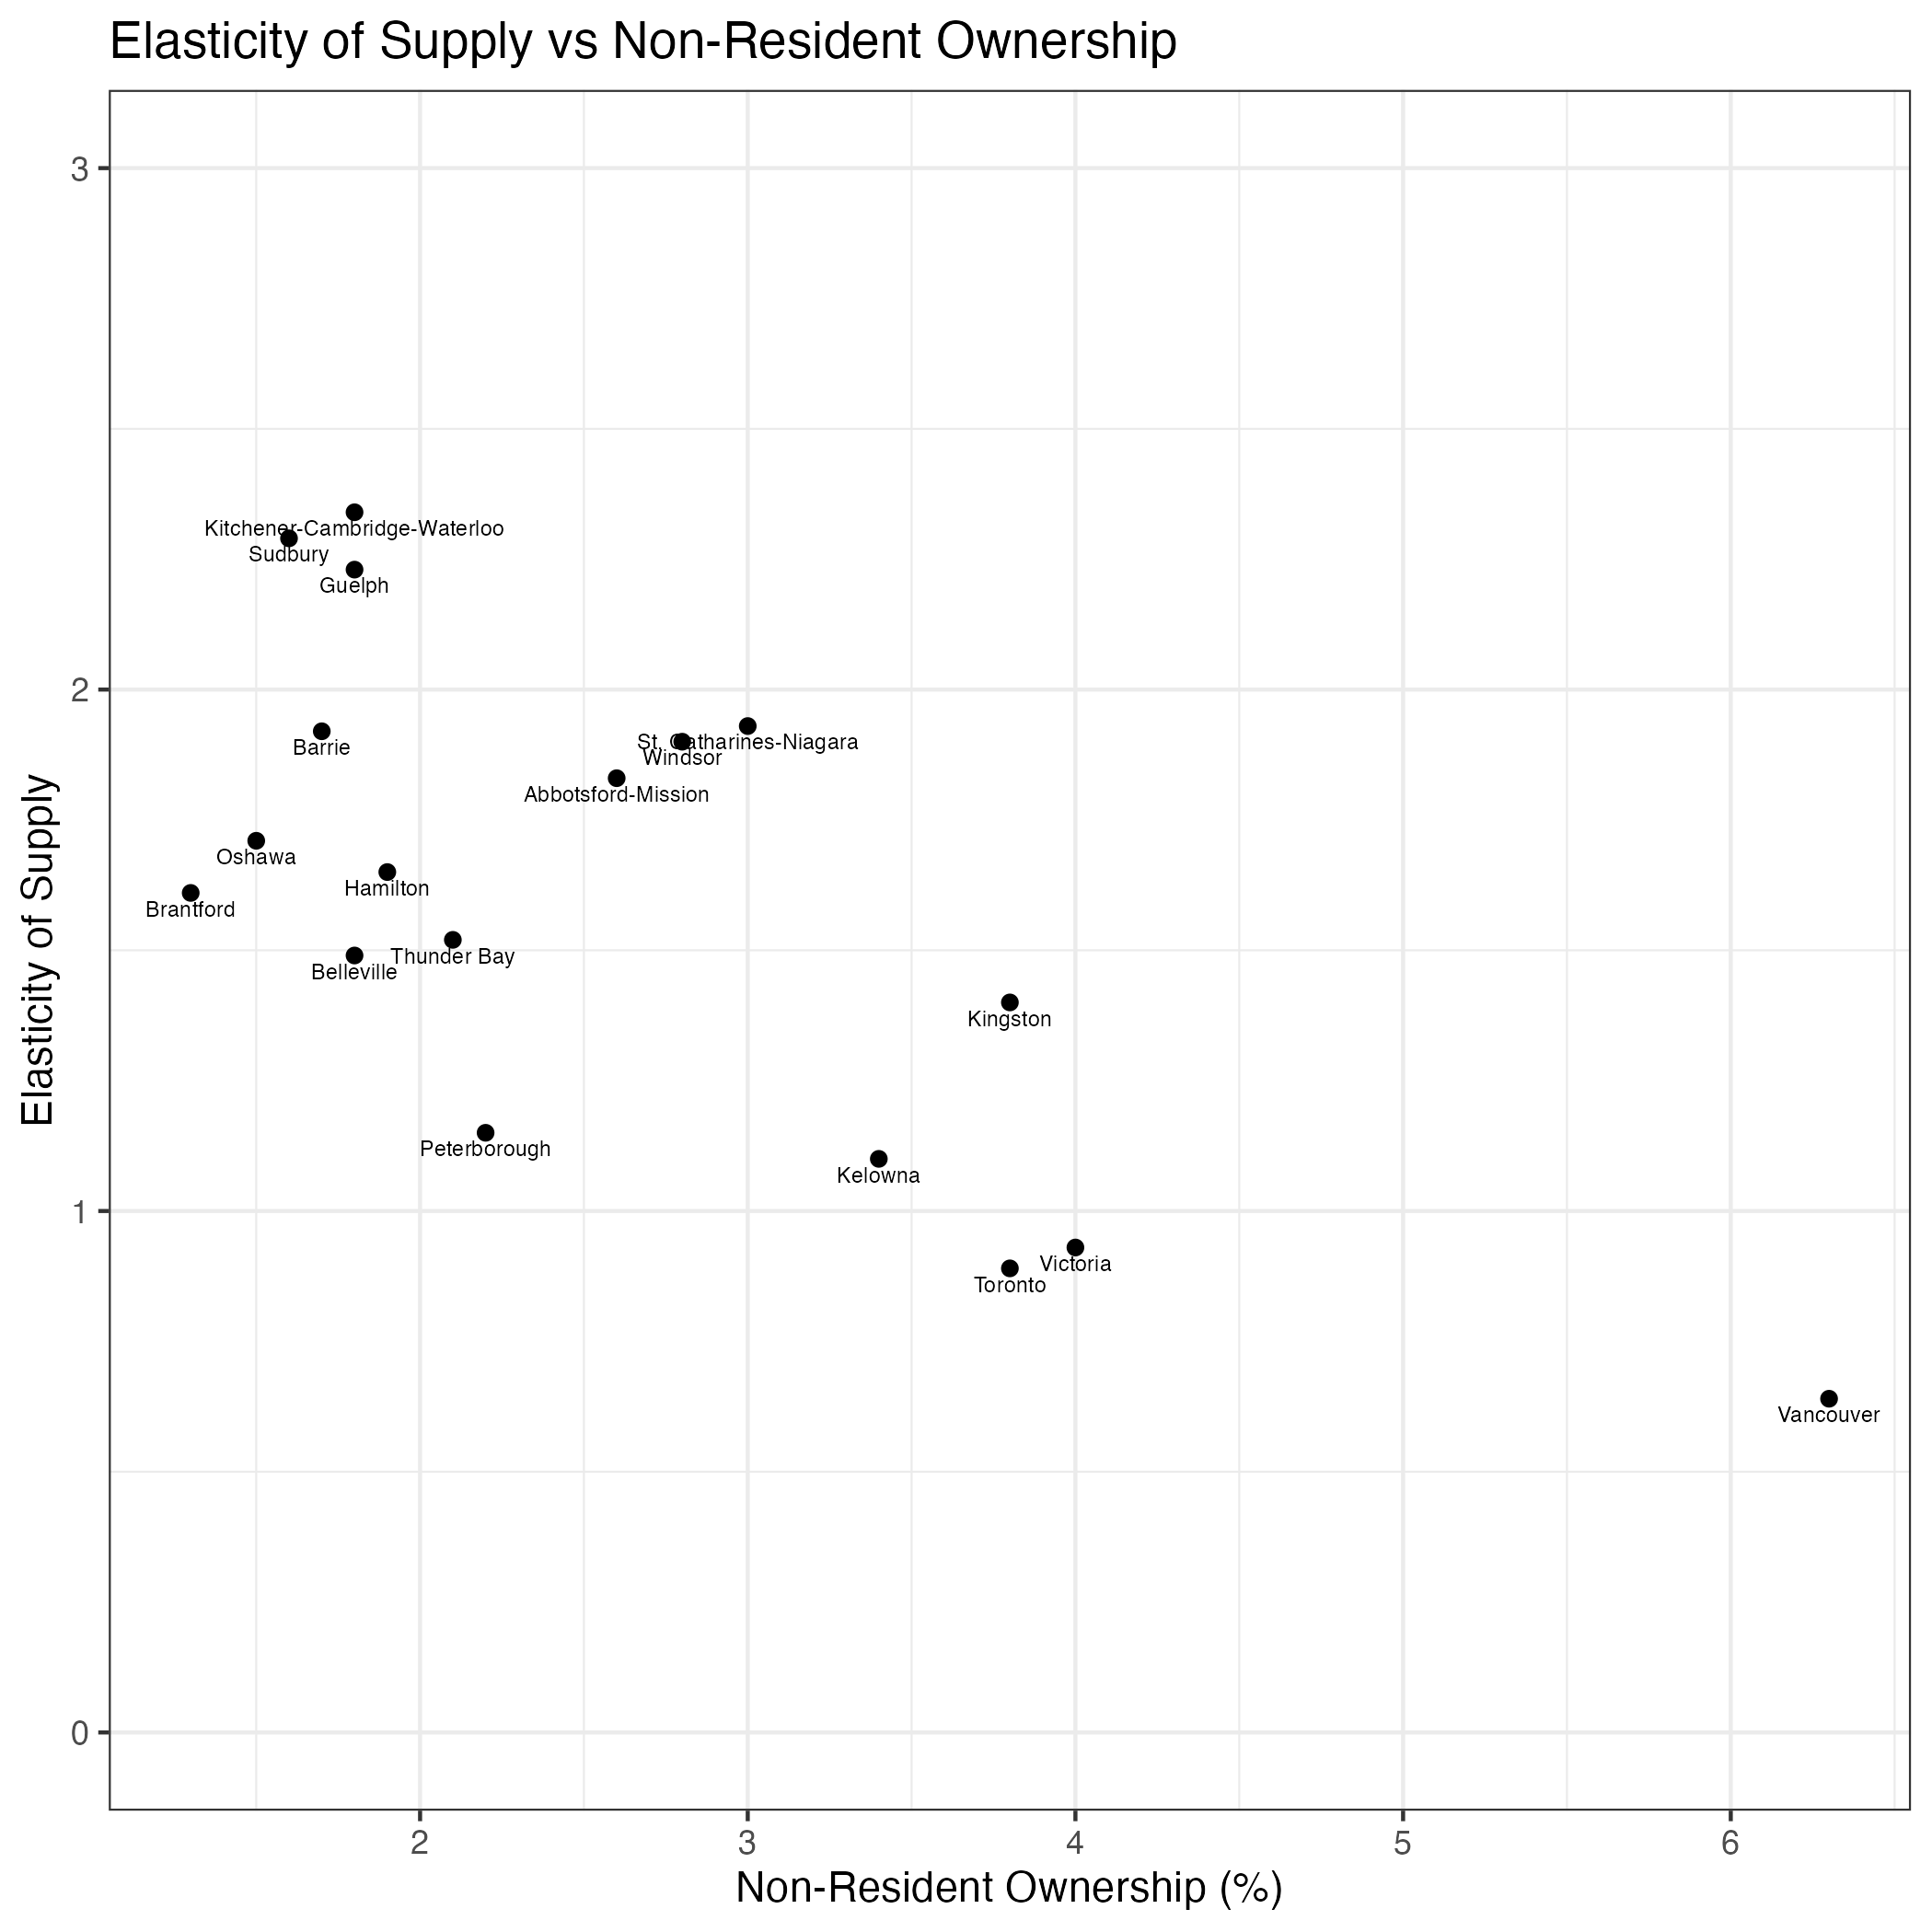
\includegraphics[width=0.8\textwidth]{"~/OneDrive - UBC/foreignImpact/text/elasticityOwnership.png"}
\caption{\label{fig:elasticityNonResident} Non-resident ownership and housing supply elasticity in Canadian CMAs. Sources: \textcite{paixao2021housing} and CHSP table ``Residency participation of residential properties, by property type and period of construction'' for 2018 estimates. (charted values of elasticities merged on CMA names by ChatGPT).}
\end{figure}

\subsection{Do foreign buyers pay more for units in the same building?}

Equation \eqref{eq:sign} suggests that foreign buyers can have a positive
supply effect when the units in which they stimulate supply are largely
occupied by locals (where $\alpha z$ is close to zero). If foreign buyers pay
higher prices than locals primarily because they occupy different buildings than
locals, it is not easy to see a positive supply effect for
locals, as these buildings will strain local contractors, increasing
construction costs.

Foreign buyers might pay more than locals for units in the same building either
by facing different prices for the same units, or by specializing in
particularly luxurious units within buildings. We cannot observe whether the
law of one price is violated, e.g.  through differential presale pricing
overseas.

There is some scope for answering the question of whether foreign buyers
purchase higher quality units within buildings than local buyers with available
data, at least for the resale market, if not for the critical presale market.
Figure \ref{fig:varianceDecomposition} uses data taken from condominium
resales in Greater Vancouver between 2010 and 2023, provided by BC Assessment.
The plot measures the year of transactions on the horizontal axis. On the
vertical axis are measures of the variance of the natural logarithm of
transaction prices by year. The red line plots the variance of all transaction
prices. The green plots the variance of mean prices across
buildings.\footnote{If there were only one transaction for each building with a
transaction in a given year, the red and green lines would coincide.} The blue
line plots the mean variance of log transaction prices within buildings. 

The dashed vertical line in Figure \ref{fig:varianceDecomposition} coincides
with the imposition of the foreign buyer tax in July, 2016. Consistent with
foreign buyers demanding more expensive units (as non-resident buyers do in the
CHSP data),\footnote{See also
\textcite{gellatlyNonresidentOwnershipResidential2017}.}  the overall variance
of prices drops sharply in the years after the tax, consistent with loss of an
important luxury segment of the market.  However, the reduction in price
variance appears to be almost entirely driven by a reduction in price variance
across buildings, rather than within buildings. This suggests that foreign
buyers did not play a large role in within-building price variance.

\begin{figure}
	\caption{\label{fig:varianceDecomposition} Variance decomposition of log resale transaction prices into total, between buildings, and within buildings, Greater Vancouver, 2010-2023. Vertical line marks implementation of B.C. foreign buyer tax in July 2016.}
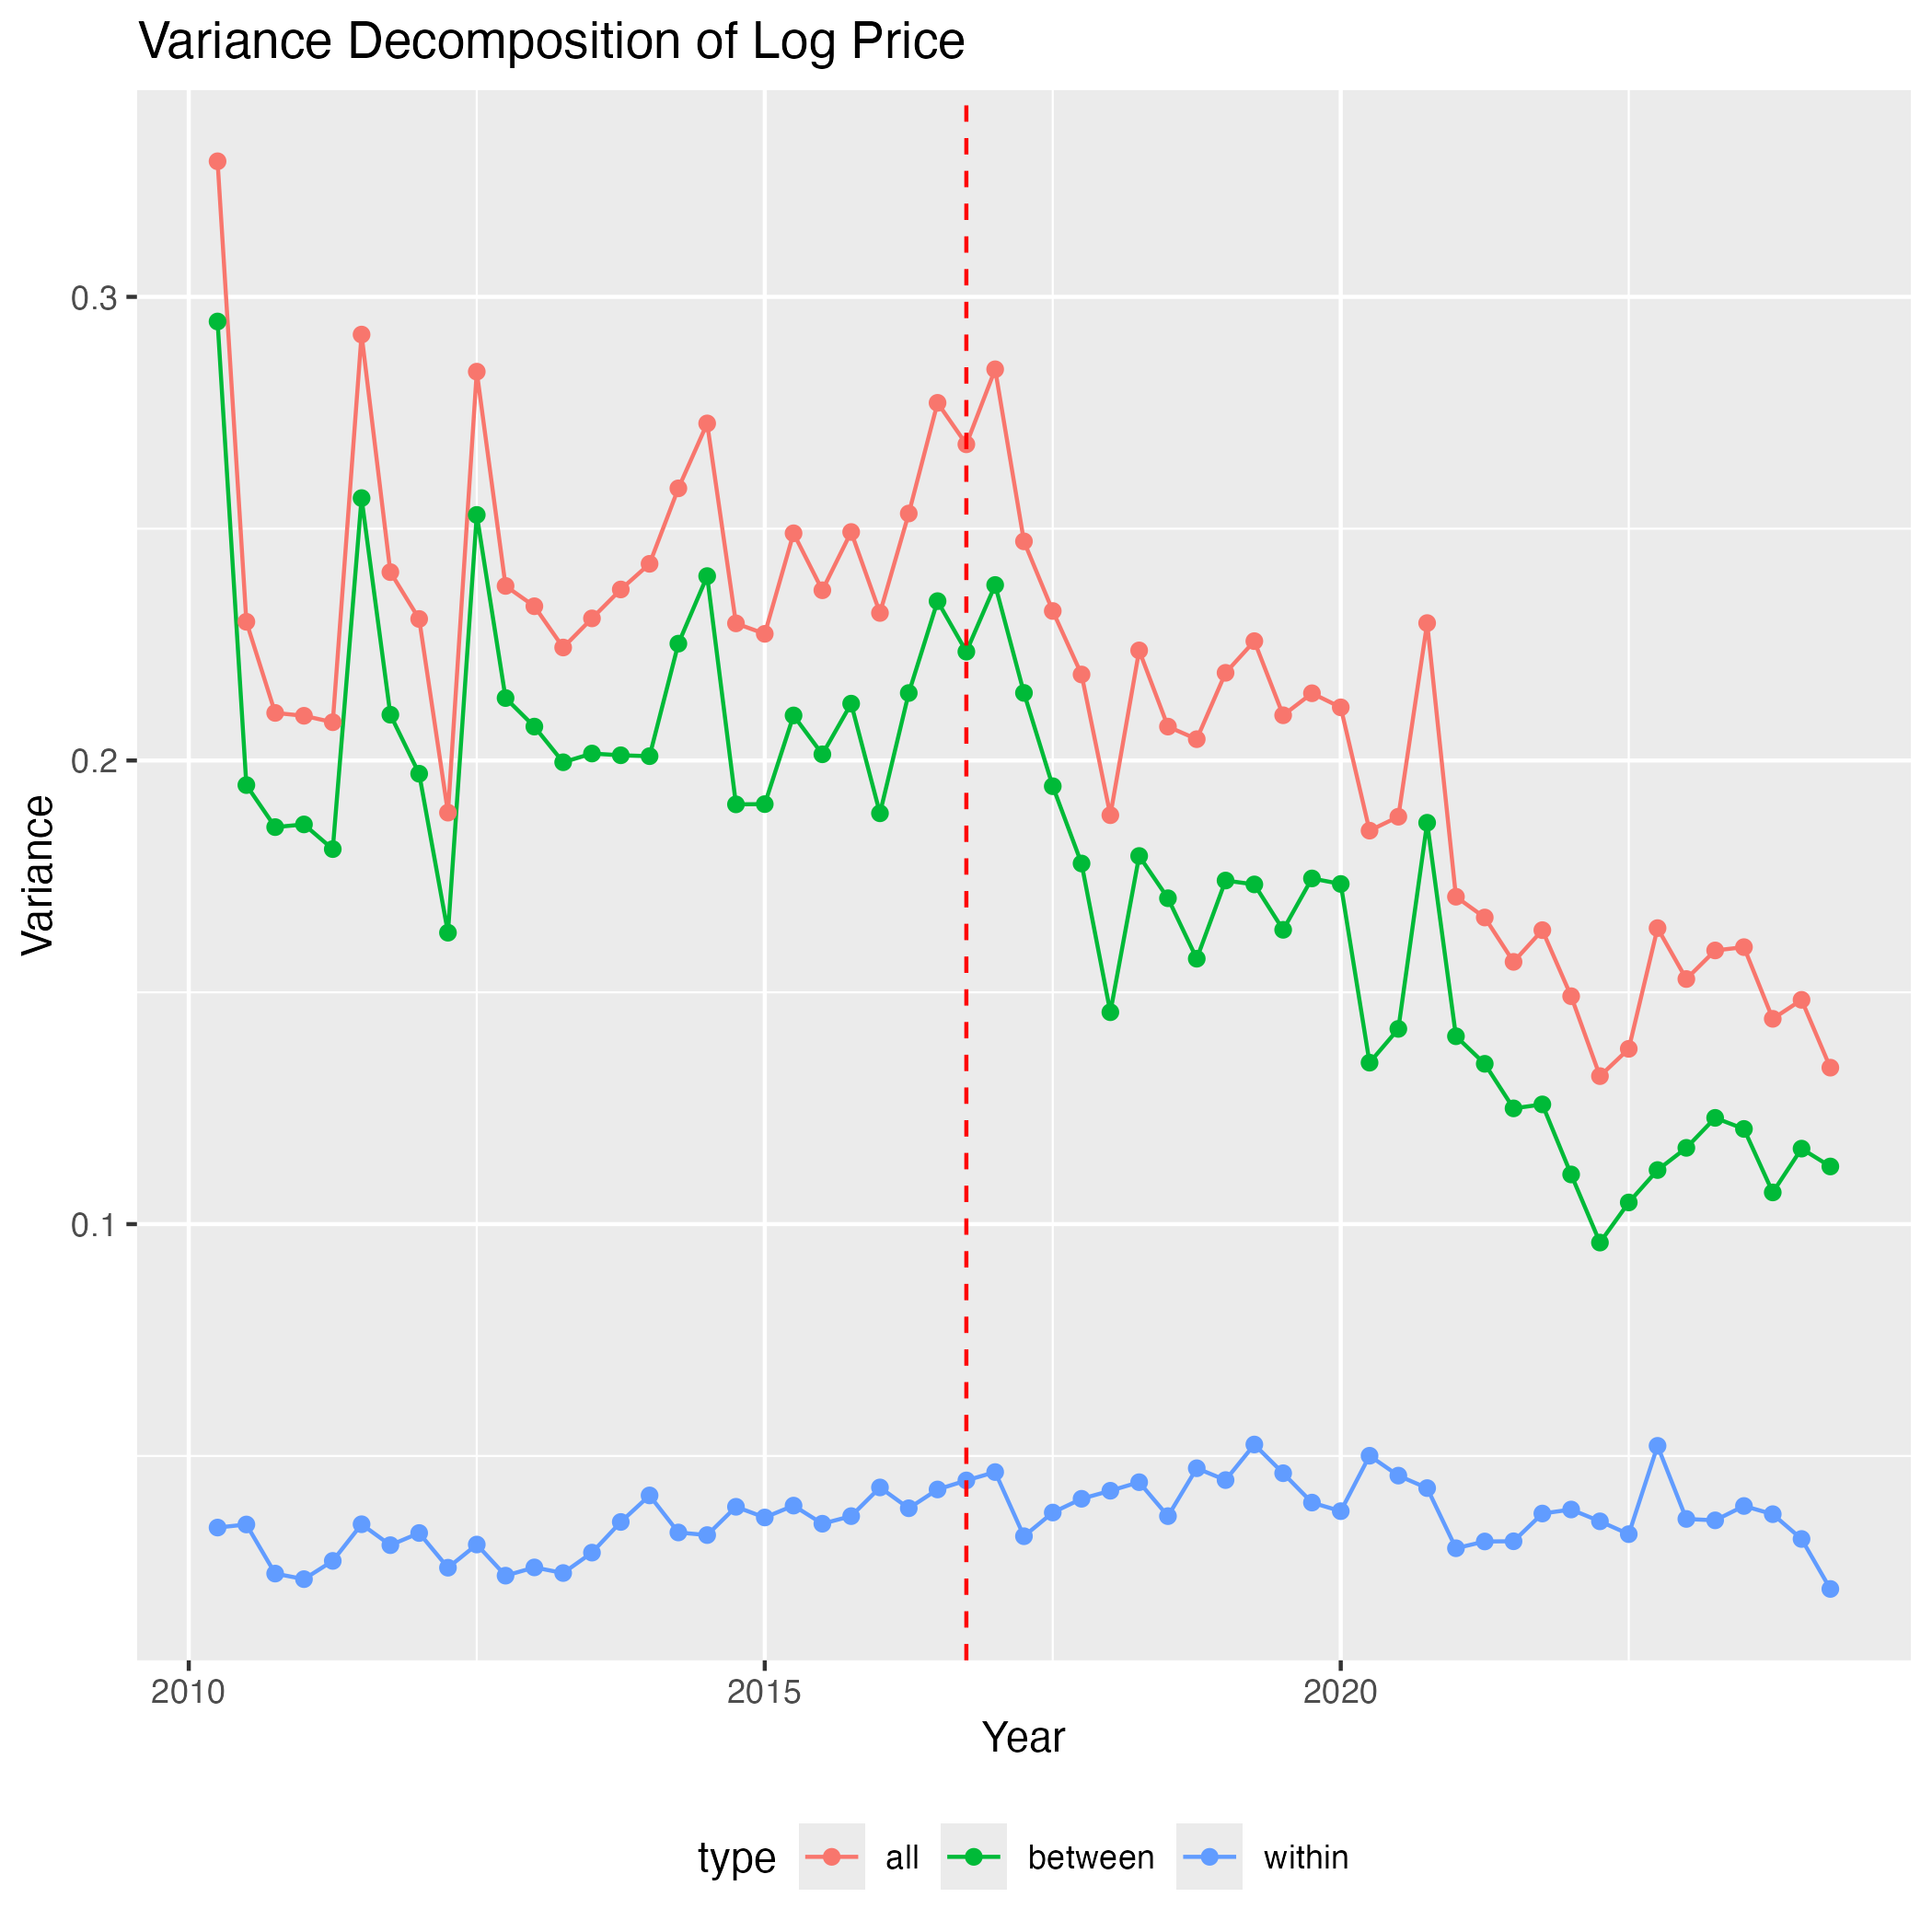
\includegraphics[width=\textwidth]{"~/OneDrive - UBC/foreignImpact/text/variance_decomposition.png"}
\end{figure}

Figure \ref{fig:varianceDecompositionNew} restricts the analysis in Figure
\ref{fig:varianceDecomposition} to transactions in buildings less than five
years old, as foreign buyers may have been concentrated in new buildings (as
non-resident buyers surely are) and new building prices may be more salient to
the presale pricing that presumably drives developer supply choices. Again,
there is little support for the notion that removing foreign buyers reduced
within-building price variation.\footnote{In both figures, there is evidence of
rising within-building price variation during the period prior to 2016 when
foreign buying was likely growing, but no clear pivot around the time of the
foreign buyer tax.}

\begin{figure}
	\caption{\label{fig:varianceDecompositionNew} Variance decomposition of log transaction prices in Greater Vancouver, 2010-2023. Same as prior figure, but transactions in buildings less than five years old at time of sale (but resale transactions only) only.}
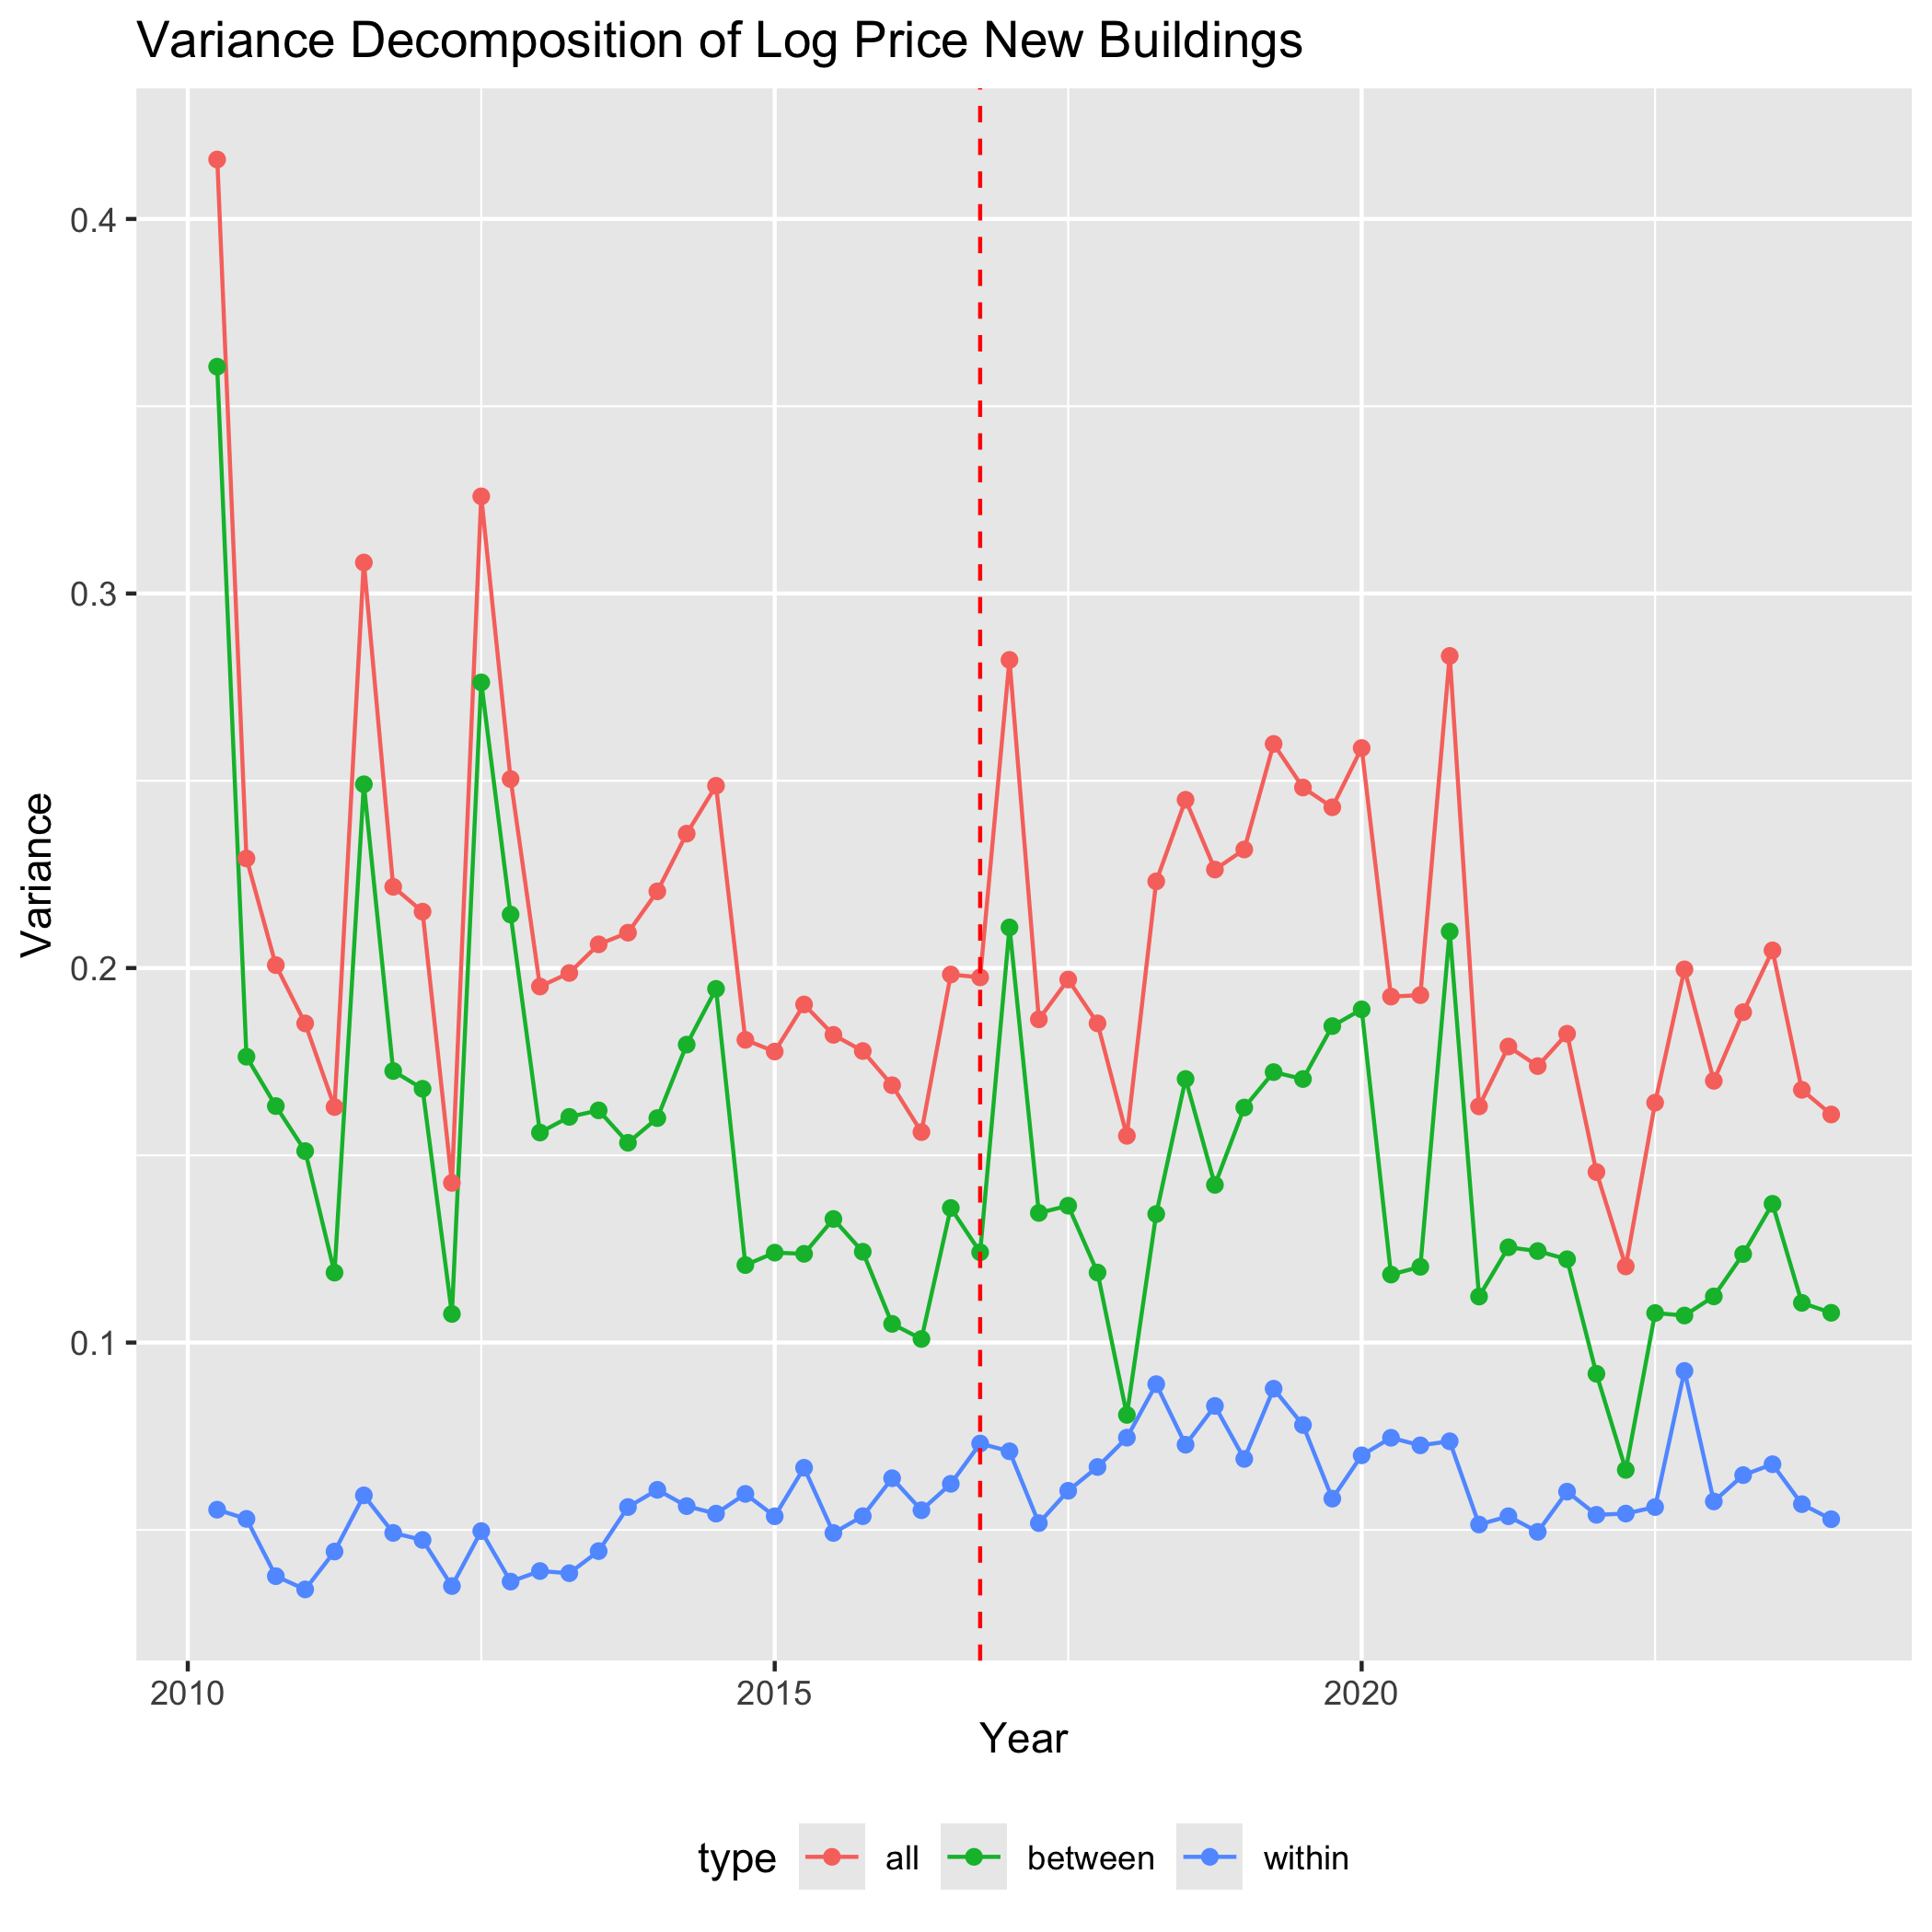
\includegraphics[width=\textwidth]{"~/OneDrive - UBC/foreignImpact/text/variance_decompositionNew.png"}
\end{figure}

Another indicator of within-building versus between price variation comes from
CHSP data comparing assessed values of properties owned by resident versus
non-resident owners. For the years starting in 2018, the Canadian Housing
Statistics Program has used its access to ownership data on the universe of
Canadian residences and their owners to publish statistics on ownership by
residency status in Canada.  Unfortunately, the stock measure is not readily
available prior to 2018 and hence prior to the implementation of B.C.'s foreign
buyer tax.  Between 2018 and 2022, the number of non-resident owners in the
Vancouver Census Metropolitan Area grew from 24,135 to 26,350, but fell as a
share of all owners from 9.6\% to 9.0\%.

While we cannot observe building-level data, we can ask what fraction of price
differences in the value of units owned by non-residents versus residents is
explained by variation across municipalities, versus within, and by
non-residents' propensity to own newer homes. Overall, among condominiums in
the Vancouver CMA, non-residents' in 2018 had a mean value of \$790,000 versus
\$630,000 for residents of Canada, a difference of over 25\%.

However, in a regression of log mean value by period of construction and
municipality on dummies for municipality, so conditioning on broad location,
the coefficient on non-resident owner versus resident owner is just .064, so
the large majority of value is explained by location. Adding dummies for ranges
of years in which buildings were completed reduces the estimated log difference
between residents and non-residents to just .017. Thus, within buildings of the
same age in the same general location, non-residents own units that are roughly
identical in value to residents, leaving little scope for extra payment for
fancier units (differences in price paid in preconstruction would not show up
in these assessed values).

The fact that non-residents own newer units than residents might be seen as a
form of differentiation in quality within buildings, in that if residents have
less willingness to pay for new units than non-residents, non-residents may
stimulate supply by paying more for new units that drive supply, leaving older
units to resident buyers over time.\footnote{A caveat is that some of the
difference in age of property owned may be attributable to non-resident
purchases growing over time. If the order of controls is reversed, in a
regression of log mean value on just period of construction dummies, the
coefficient on non-resident ownership is -.065, so the difference in condo age
explains as much of the value difference as municipality, and is unlikely to be
mostly explained by differential dates of purchase.}

Importantly, CHSP statistics are an approximation (possibly biased) of foreign
ownership, because some owners who live overseas are Canadian citizens or
permanent residents, and hence exempt from foreign buyer taxes. Also, some
Canadian residents are not yet landed immigrants, and hence are subject to the
foreign buyer tax. 

\subsection{Stock and flow of foreign purchases in Greater Vancouver}

When the share of foreign buyers $\alpha$ is small, so that most homes are
purchased (and occupied) by locals, any inducement to build by foreign buyers
paying premium prices (possibly for premium apartments in less demand among
locals) is likely to be positive for local affordability.

The apparent declining stock of foreign ownership as a share of all residences
(as proxied by residency) is matched by a declining share of the flow into
ownership. The B.C. provincial government started collecting data on the
nationality of residential property buyers shortly before implementing the
additional property transfer tax of 15\% on foreign buyers in mid-2016. In the
month (July) prior to implementation, 15\% of purchases in Metro Vancouver
involved foreign participation. For the years since, the fractions have been as
shown in Table \ref{tab:fbt}. COVID and the national foreign buyer ban have
likely contributed to the decline over time in foreign participation.

\begin{table}
	\caption{\label{tab:fbt} Fraction of residential transactions in Metro Vancouver with foreign participation, per B.C. Property Transfer Tax data. Source: \texttt{https://catalogue.data.gov.bc.ca}}
	\begin{tabular}{lc}
		\hline
		Year & Fraction of transactions with foreign participation \\
		\hline\hline
		2017 & 3.7\% \\
		2018 & 2.9\% \\
		2019 & 2.0\%\\
		2020 & 1.4\%\\
		2021 & 1.1\%\\
		2022 & 1.3\%\\
		2023 & 0.9\%\\
		2024 & 0.9\%\\
		\hline
	\end{tabular}
\end{table}

\subsection{Are foreign buyers' homes left homes empty?}

The variable $z$ in equation \eqref{eq:sign} represents the fraction of
foreign-owned homes that are not occupied by locals, either because they are
used as secondary residences by foreign buyers, or government puts low weight
on housing for not-yet-landed immigrants. When this fraction is larger, foreign
buying is less helpful to affordability. It is difficult to know what fraction
of the stock represents primary residences for not-yet-landed immigrants, but
the fraction of homes left empty most of the year is measured by nationality
status by the B.C. Finance Ministry as part of administration  of the
Speculation and Vacancy Tax.

Owners of homes that are not primary residences are subject to extra taxes in
certain jurisdictions in Ontario and B.C., and foreign owners of Canadian homes
left vacant more than half of a year are subject to a federal ``Underused
Housing Tax.'' In Vancouver, there is a third, municipal empty homes tax. If
these taxes are high enough, units will be rented or sold to locals (such that
$z$ is close to zero), or the tax revenue should be sufficient to leave local
residents better off than if the unit were owned by a local. However, if empty
home taxes are set at a sufficiently low level, foreign owners may leave homes
empty, and the tax revenue may not be sufficient to compensate locals for the
loss of housing stock.

In the presence of the B.C. empty homes tax regime, foreign, non-resident
owners who retain their properties most commonly rent them out to locals. Per
\textcite{specTax2019}, of 3,709 foreign owners deemed subject to the empty
homes tax in 2018 in B.C., a large majority no longer held empty homes in 2019.
1,205 of these foreign owners subject to the Speculation and Vacancy tax
transitioned to renting their homes out in 2019, 1,413 sold their property, 951
remained subject to the tax, and 66 transitioned to using the home as a primary
residence. Perhaps through ``burnout'' just over half of 1,308 foreign owners
deemed subject to the tax in 2020 remained subject to the tax in 2021. Overall,
for the 2021 tax year, roughly 5.5\% of declared foreign owners homes' were
deemed empty. Of the remaining 94.5\%, it is not clear what fraction correspond
to the non-local measure $z$: whether a non-permanent resident living a home
regularly should be deemed part of the local demand curve is a political
question.

\subsection{Back-of-the-envelope calculations of foreign buyer effects on affordability}

With a rough idea of plausible magnitudes of key parameters in equation
\eqref{eq:sign} in hand, we can perform back-of-the-envelope calculations
suggestive of the net effect of foreign buying on housing affordability for
locals in the Greater Vancouver context. As described above, the magnitude of
the product of three terms governs being greater than or less than one
determines whether a small increase in foreign buying improves or worsens local
affordability, per equation \eqref{eq:sign}. 

For Greater Vancouver, at \textcite{paixao2021housing}'s estimate of a supply
elasticity of .65, the product of the terms representing the premium paid by
foreign buyers and domestic occupancy intensity in equation \eqref{eq:sign}
would have to be roughly 1.5 or greater to yield a positive effect of foreign
buyers on local prices. We do not know either of the components of that
product, but there is evidence that the foreign buyer premium within buildings
is not large on account of purchase of different units. Also, foreign buyers
represented roughly 15\% of the market over a sampled period prior to
implementation of B.C.'s Foreign Buyer Tax. At a 10\% foreign buyer premium and
$1-\alpha=.85$, the local occupancy of foreign-owned units $z$ would have had
to have satisfied:

\begin{align}
	\underbrace{.65}_{\text{Vancouver supply elasticity}} \underbrace{\times .1}_{\text{modest foreign price premium}} \times \underbrace{\frac{1-.15 z}{z}}_{\text{Domestic occupancy}} \geq 1\\
	 z \leq \frac{.65 \times .1}{1+.65 \times .1} \approx .06
 \end{align}

Notably, even with the speculation and vacancy taxes in B.C., in 2021, roughly 5.5\% of foreign-owned homes were deemed empty. Suggesting roughly zero local affordability effect of foreign buying at the pre-foreign buyer tax levels of investment, and a modestly positive effect with almost no foreign buying. This suggests that one, but not both of a foreign buyer tax or a vacancy tax is required to avoid adverse foreign buying impacts on local affordability.

\section{Conclusion}

A simple model of foreign purchases reinforces natural intuitions that foreign
buyers can act to stimulate supply, and thus enhance affordability for locals
when the foreign buyers are a small part of the market, when they pay 
much more than local residents would for homes in the same buildings, when
housing supply is elastic with respect to price, and when a large fraction of
foreign-purchased homes are rented to locals or sold soon after buildings are
constructed. In this framework, preconstruction purchases by foreign (or
domestic) buyers followed by assignment to local buyers prior to completion
should have purely positive affordability effects, so ``flipping'' taxes such
as B.C.'s should presumably exempt presales.

Foreign buyers in Canada are concentrated in housing markets with relatively
low supply elasticities, and most of the variation in the value of apartments
owned by non-residents is explained by location and building age, not different
unit quality. These facts suggest that in the absence of empty homes taxes,
foreign buyers are unlikely to provide little affordability benefit to locals
through a net supply channel, unless they face significant price discrimination
in the preconstruction market. However, in the presence of empty homes taxes,
the large majority of foreign owners appear to either use homes year round,
rent them to locals, or sell. Empty homes taxes thus seem likely sufficient to
avoid adverse affordability effects of foreign ownership and in their presence
it is not out of the question that taxes or restrictions on foreign buying may
harm affordability.

\printbibliography

\end{document}
